\subsection{Newton-Cotes Integration - Chapter 21}

\begin{enumerate}

  \item {\bf The Standard Reimmann Sum}

    The standard Reimmann sum can be used to integrate equations. For
    example, assume for the moment that the velocity of a ball in
    free-flight is equal to $v(t) = v_0 + at$. In calculus it is shown
    that the area under the curve $v(t)$ is equal to the
    position. That is,

    \begin{equation}
      x(t) = x_0 + \int\limits_{t=0}^t v(t) dt \approx x_0 + \sum\limits_{i=1}^N
      v(t_i) \Delta t
    \end{equation}

    The position is merely the integral of the velocity curve. In
    addition, the position can be approximated by the area under the
    curve using a series of rectangles to approximate the area under
    the curve. Note that the equation above is a similar representation
    or for Euler's method. That is, Euler's method is a first order
    method for integrating equations of motion and a Reimmann sum is a
    zero-order method for obtaining the area under the curve.

  \item {\bf Car Example}

    So let's say we're driving our care and we take a few measurements
    as we head to work. We also note the time when we take the
    measurement.

    \beq
    \begin{matrix}
    V = [30,35,0,0,50,50,0]~mph \\
    T = [10,15,16,17,20,25,30]~min\\
    \end{matrix}
    \eeq

    The solution to this problem is then given by using the Reimann
    Sum. Note that we are using the left Reimann sum since we assume
    that the initial velocity and time are both zero.

    \beq
    X = V_0(T_0-0) + V_1(T_1-T_0) + \hdots + V_N(T_N-T_{N-1})
    \eeq

    \beq
    X = (30*(10-0) + 35*(15-10) + 0*(16-15) + 0*(17-16) + 50*(20-17) +
    50*(25-20) + 0*(30-25))/60
    \eeq
    
    Which results in about 14.58 miles. We divide by 60 because our time is in minutes and our velocity is
    in miles/hour. This solution can be visualized in the graphic
    below.
    
    \begin{figure}[H]
      \begin{center}
        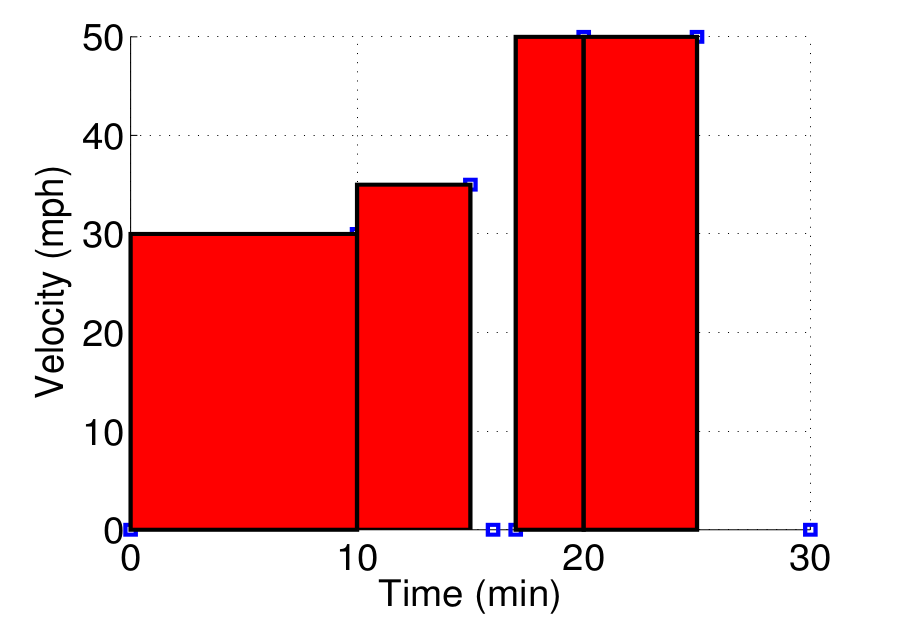
\includegraphics[height=0.5\textwidth,width=0.7\textwidth]{Graphics/Reimmann}
      \end{center}
    \end{figure}

    Notice though that there is quite a bit of error. It is possible
    to reduce the error by taking more measurements thus reducing
    $\Delta t$.

  \item {\bf Round-Off Error}

    The equation above has a very fundamental term in the equation
    above and that is the timestep ($\Delta t$). The solution becomes
    more approximate as the timestep decreases. This reduction in the
    timestep and the increase in accuracy is known as round-off
    error. As the timestep becomes smaller and smaller you reduce the
    amount of round off error in your system because more decimal
    places are used in the approximation. Note, however that there is
    a limit to how small you can make the timestep. If the timestep is
    reduced to levels below the threshold of your computer you will
    find that the error in your estimate actually begins to
    increase. This limit is known as the limit of precision. That is,
    the CPU cannot be more precise given the timestep you have chosen
    and the value of your error begins to rise.

    \begin{figure}[H]
      \begin{center}
        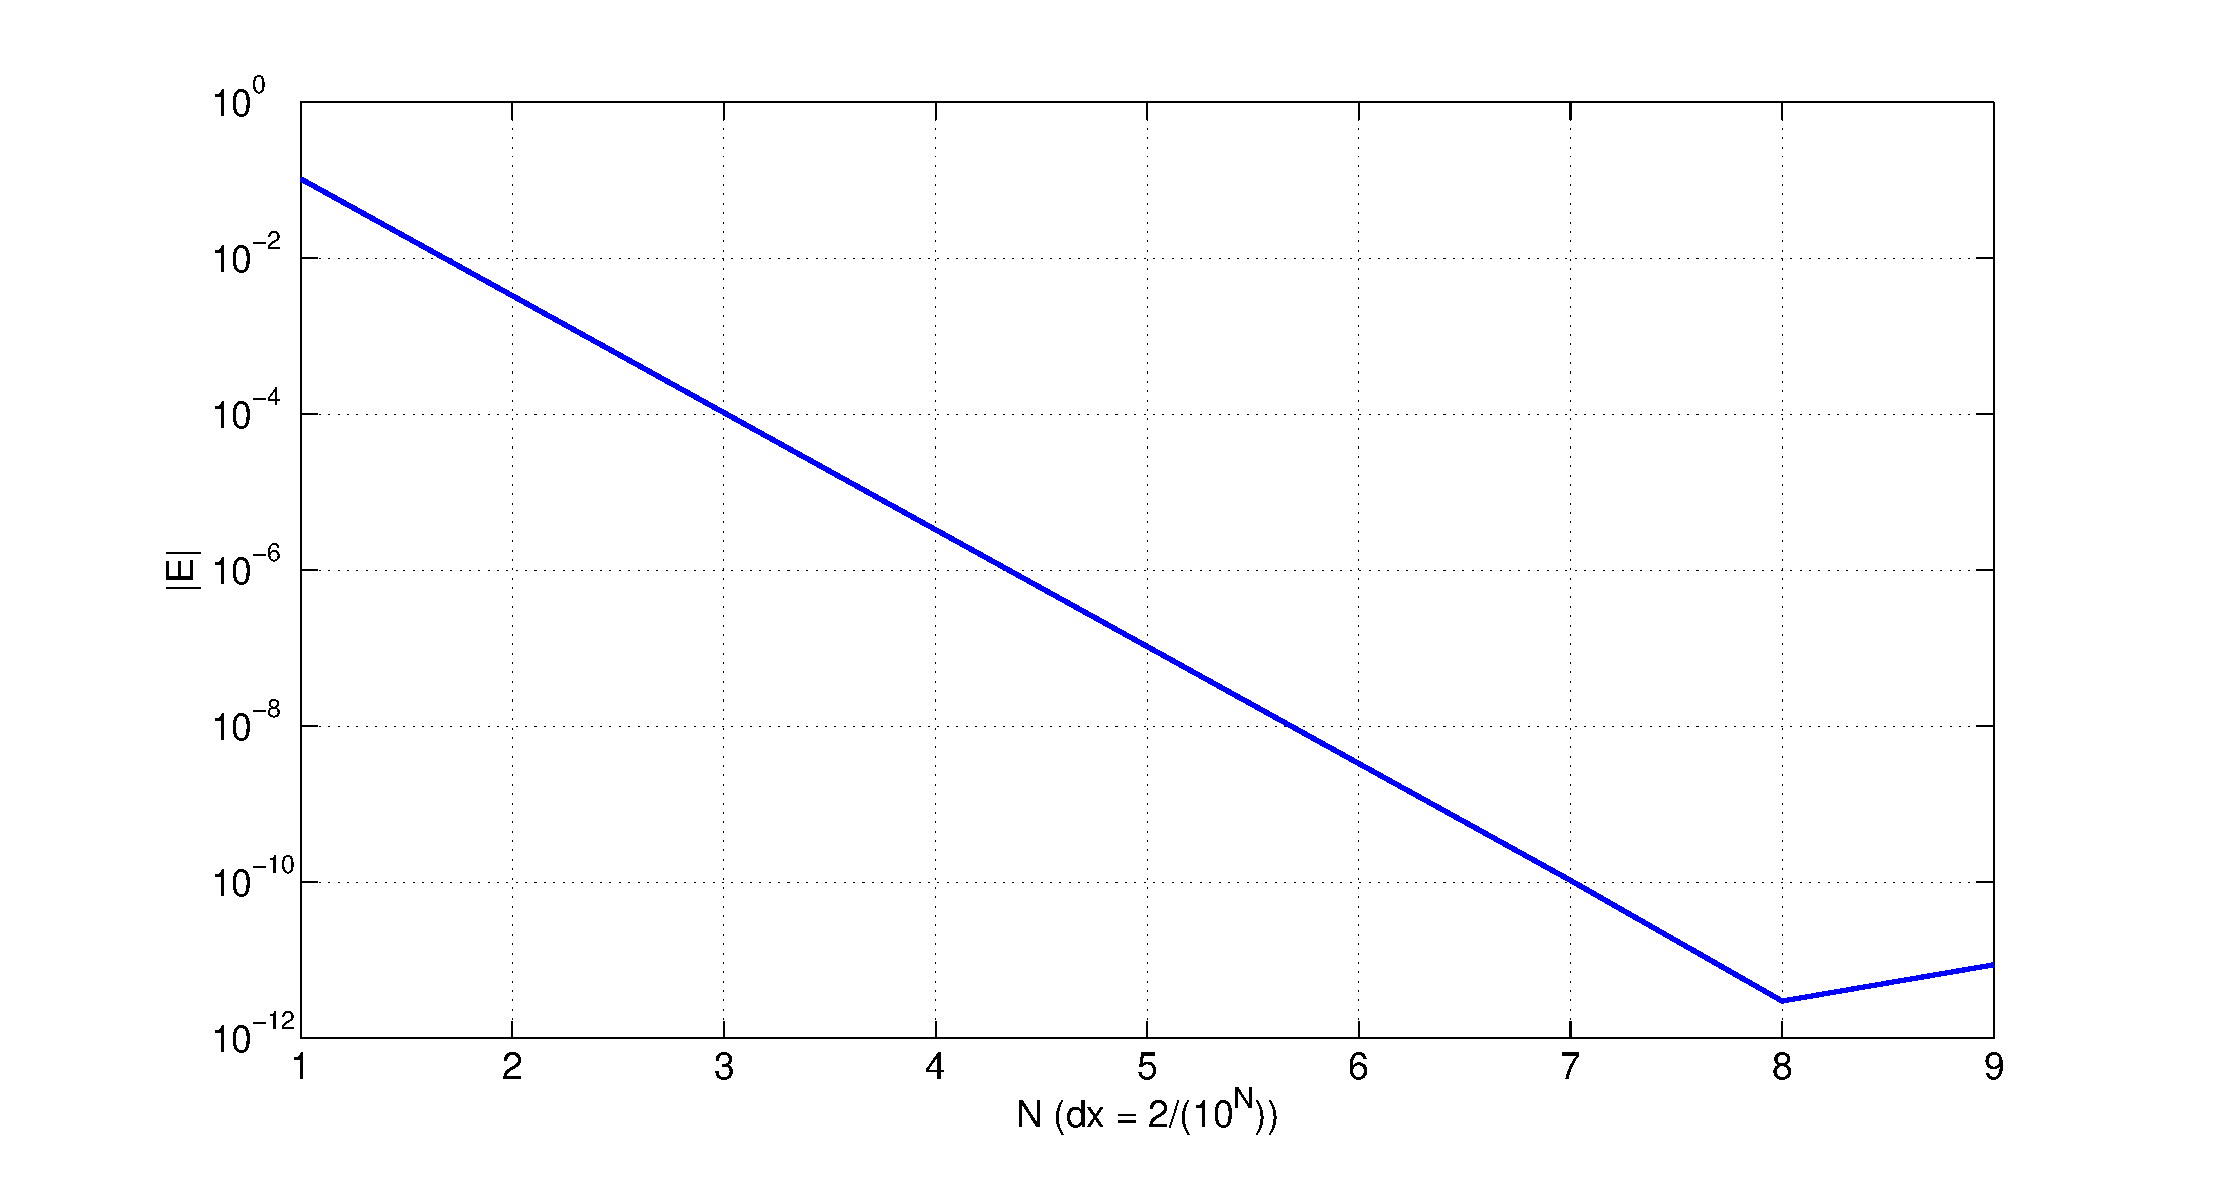
\includegraphics[height=0.5\textwidth,width=0.7\textwidth]{Graphics/Limit_Of_Precision}
      \end{center}
    \end{figure}

    However, in our example above with the car driving, we cannot
    decrease $\Delta t$ because we only have a discrete set of
    measurements. Instead we can increase the order of our method.

\item {\bf Trapezoidal Rule}

  Similar to the Reimmann Sum the trapezoidal rule sum individual
  Trapezoids instead of rectangles. The area of a trapezoid is given
  by $(1/2)(b_1 + b_2)h$. Where b is the base and h is the width. For
  our integration of functions we have 

  \begin{equation}
    I \approx \sum\limits_{i=1}^{N}\frac{1}2 (f(t_i)+f(t_i+\Delta
    t))\Delta t
  \end{equation}

  Note that the Standard Reimmann sum is a zero order approximation
  whereas the trapezoidal rule is a linear or first order
  approximation. Because the trapezoidal rule is a first order
  approximation, errors are still produced but they are not as bad.

\item {\bf Car Example Returned}

  Let's return to the car example. Instead of adding rectangles let's
  use trapezoids and add them together using the trapezoidal rule. The
  graphic below depicts the solution using trapezoids. Notice how much
  error is reduced when using trapezoids instead of rectangles. I've
  placed the Reimman Sum and Trapezoidal rule problem side by side to
  show the benefit.

  \begin{figure}[H]
    \begin{center}
      \begin{tabular}{cc}
      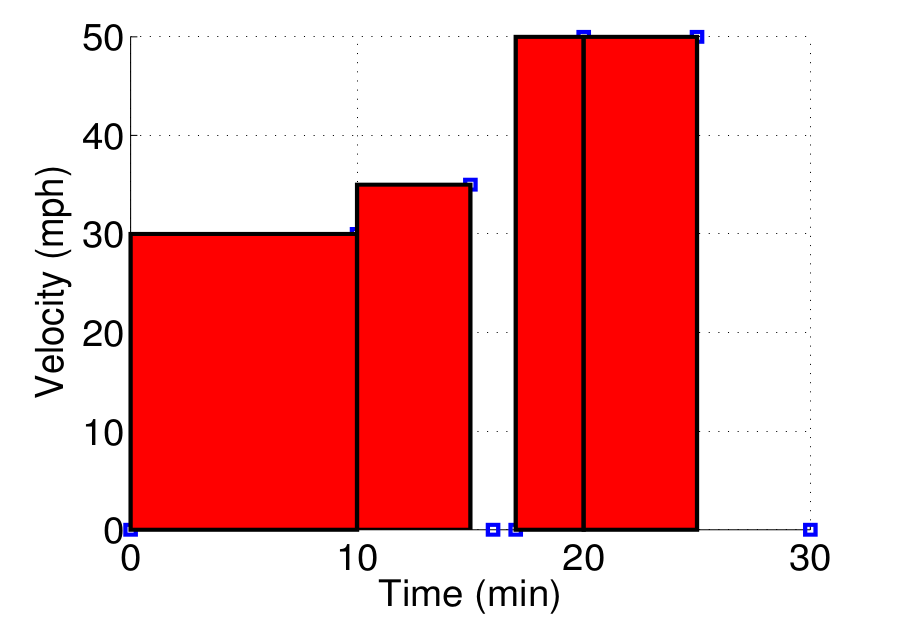
\includegraphics[height=0.3\textwidth,width=0.4\textwidth]{Graphics/Reimmann} &
      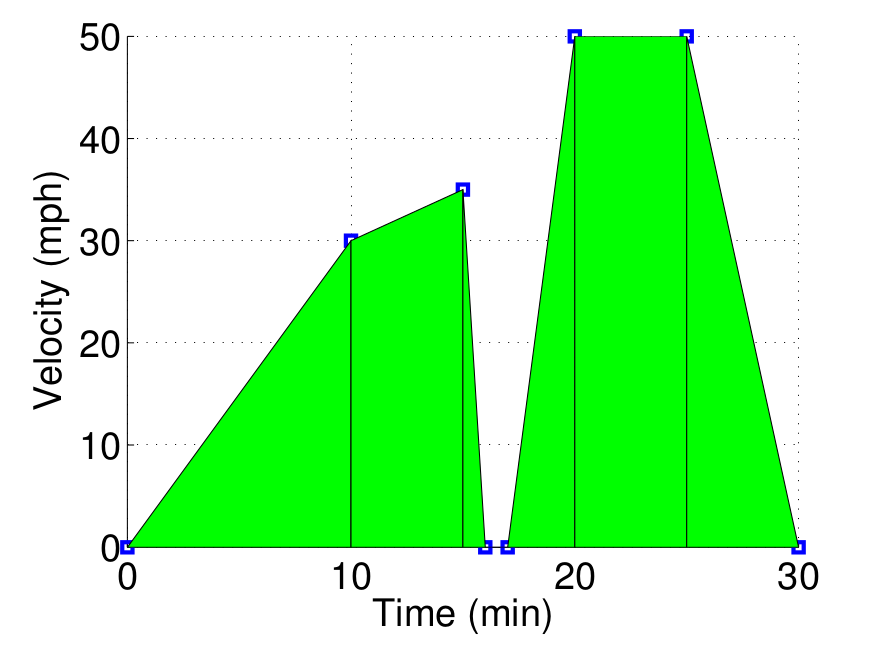
\includegraphics[height=0.3\textwidth,width=0.4\textwidth]{Graphics/Trapezoidal}
      \end{tabular}
    \end{center}
  \end{figure}

  The solution of adding the triangles is realized in the equation
  below.

  \beq
  \begin{matrix}
  X = \frac{1}{2}(V_0+V_1)(T_1-T_0) + \frac{1}{2}(V_1+V_2)(T_2-T_1) +
  \hdots + \frac{1}{2}(V_N+V_{N-1})(T_N-T_{N-1})\\
  \ \\
  X = \frac{1}{2}((0+30)(10-0) + (30+35)(15-10) + (30+35)(15-10) + \\
  (35+0)(16-15) + (0+50)(20-17)+ (50+50)(25-20) + (50+0)(30-25))/60
  \end{matrix}
  \eeq

  The solution to using the trapezoidal rule is 15.71 miles which is
  alot different than the Reimman sum solution.
  
\item {\bf Compute Truncation Error of Trapezoidal Rule}

  The trapezoidal rule is not perfect though. The figure below shows the inherent problem of using the
  trapezoidal rule for functions with a second derivative. That is,
  the order of the system is larger than 2.
  
  \begin{figure}[htb]
    \begin{center}
      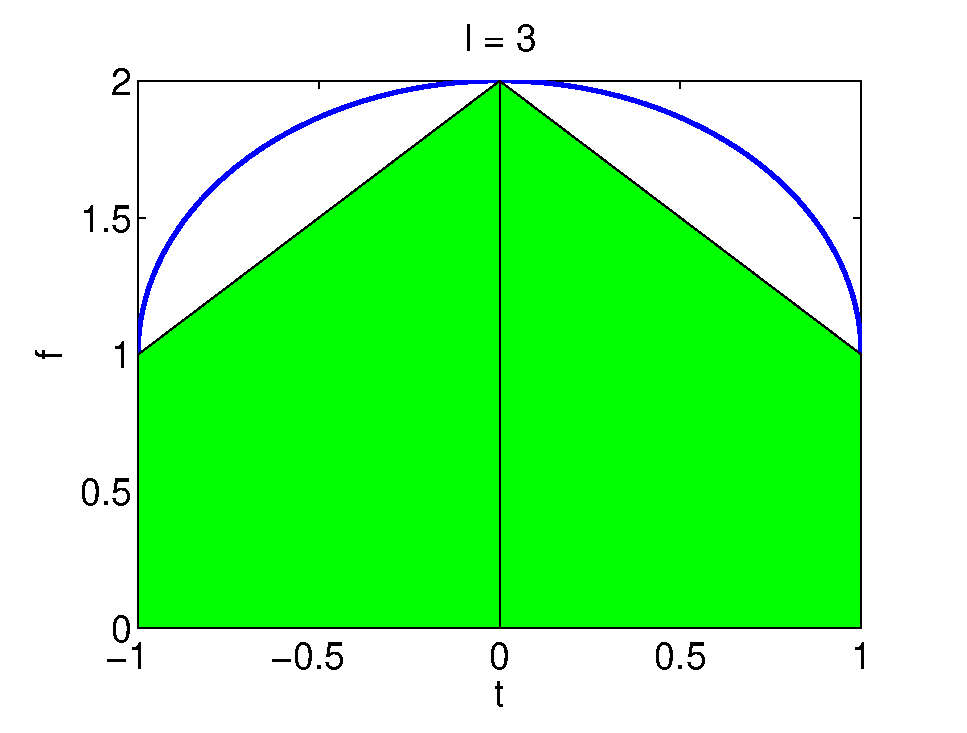
\includegraphics[height=0.45\textwidth,width=0.6\textwidth]{Graphics/Truncation_Error}
    \end{center}
  \end{figure}
  
  Here the green shaded region can be defined as the area of the
  trapezoid. The blue line is the analytical solution thus the white
  region is the error created by the trapezoidal rule. In a general
  sense the truncation error can be written using the following
  equation below.
  
  \begin{equation}
    E_{Ti} = \int\limits_{a}^{b}f(t)~dt - \frac{1}2(b-a)(f(a)-f(b))
  \end{equation}

  As noted previously it is possible to write f(t) as a taylor series
  expansion and evaluate the first integral. Doing this yields the
  equation below.

  \begin{equation}
    E_{Ti} = \frac{-1}{12} f''(\zeta)(b-a)^3
  \end{equation}

  Remember from Chapter 4 that $\zeta$ is a number in
  between the interval a,b. The total error than for the trapezoidal
  rule is then just the sum of all errors. Note that $\Delta x = (b-a)$.

  \begin{equation}
    E_T = \sum\limits_{i=1}^N E_{Ti} = \sum\limits_{i=1}^N
    \frac{-1}{12} f''(\zeta)\Delta x^3
  \end{equation}

  Making the substitution that $\Delta x = (B-A)/N$ where A and B are
  $x_1$ and $x_N$ respectively the total error is written as

  \begin{equation}
    E_T = \frac{-1}{12 N^2} \bar{f}''(B-A)^3
  \end{equation}

  Here $\bar{f}''$ is the average second derivative over the interval
  A,B.

  \item {\bf Simpson's 1/3 and 3/8 Rule}
    
    Clearly it is possible to fit a polynomial much like the RK2
    techniques and the taylor series expansion. Fitting second order
    and third order polynomials yields Simpson's 1/3 and 3/8 rule.

    \begin{equation}
      I \approx = \sum\limits_{i=1}^N \frac{1}6 (f(t_i) + 4
      f(t_i+\Delta t/2) + f(t_i + \Delta t))\Delta t
    \end{equation}

    \begin{equation}
      I \approx = \sum\limits_{i=1}^N \frac{1}8 (f(t_i) + 3
      f(t_i+\Delta t/3) + 3f(t_i+2\Delta t/3) + f(t_i + \Delta t))\Delta t
    \end{equation}
    
  \item {\bf Improper Integrals}

    Improper integrals pose a problem for numerical integration becase
    there is a $\infty$ in the integral. For example,

    \begin{equation}
      I = \int\limits_{0}^{\infty}f(t)dt
    \end{equation}

    Numerically, $\infty$ does not exist. A computer can represent a
    very large number but it cannot represent $\infty$. Thus, the
    solution is to convert the integral to two integrals.

    \begin{equation}
      I = \int\limits_{0}^{B}f(t)dt + \int\limits_{B}^{\infty}f(t)dt
    \end{equation}

    In order to remove the $\infty$ in the second integral a change of
    variables is done such that $x=1/t$. Going through the change of
    variables yields the following equation.
    
    \begin{equation}
      I = \int\limits_{0}^{B}f(t)dt + \int\limits_{0}^{1/B}\frac{1}{x^2}f(1/x)dx
    \end{equation}

    Now the two integrals above can be evaluated with two separate
    numerical integration schemes.

\end{enumerate}
